\apendice{Especificación de Requisitos}

\section{Introducción}
En este anexo se voy a comentar un apartado esencial en el desarrollo de un elemento software, esto es los requisitos funcionales y los casos de uso, ya que representan lo que tiene que ser y/o hacer nuestra aplicación, programa o proyecto en general. Estos conceptos son definidos por el usuario con ayuda de los diseñadores del software, para definir, desde el primer momento, lo que tiene que hacer el software a desarrollar.
\section{Objetivos generales}
Los objetivos generales, expuestos y debatidos en las primeras reuniones con APACE, son los siguientes:
\begin{itemize}
	\item Poder capturar datos con los que poder realizar la investigación.
	\item Interpretar las emociones de los pacientes a partir de grabaciones de audio y unas opciones adicionales.
	\item Interpretar las respuestas de los pacientes a partir de grabaciones de audio.
	\item Toda aplicación desarrollada ha de ser simple y accesible.
\end{itemize}
\section{Catalogo de requisitos}
En esta sección voy a comentar los requisitos funcionales y no funcionales del proyecto.
\subsection{Requisitos funcionales}
\begin{itemize}
	\item \textbf{RF-1 Selección del paciente:} las aplicaciones deben permitir la selección de los pacientes permitidos.
	\begin{itemize}
		\item \textbf{RF-1.1 Visualización de los pacientes:} en las aplicaciones se tiene que poder ver la lista de posible pacientes a seleccionar.
		\item \textbf{RF-1.2 Paciente seleccionado único:} solo se puede seleccionar a un paciente a la vez.
		\item \textbf{RF-1.3 Permanencia del paciente:} en las aplicaciones una vez que se ha seleccionado un paciente este sigue a lo largo de la ejecución, sin variar por ningún tipo de error.
		\item \textbf{RF-1.4 Paciente por defecto:} en la aplicación de interpretación tiene que poder cargarse un paciente por defecto que aparezca seleccionado al abrir la aplicación.
	\end{itemize}
	\item \textbf{RF-2 Selección de emociones/respuestas:} en la aplicación de recogida de datos, el usuario tiene que poder seleccionar las emociones o respuesta relacionado con el sonido que acaba de grabar.
	\begin{itemize}
		\item \textbf{RF-2.1 Selección de emociones o respuesta}: en la aplicación de generación de datos, el usuario solo puede elegir como resultado de la grabación varias emociones o una respuesta, no puede elegir valores de ambos campos.
		\item \textbf{RF-2.2 Selección de sí o no:} en la aplicación de generación de datos, si elegimos como resultado una respuesta esta ha de ser sí o no, pero no se puede seleccionar ambas a la vez.
		\item \textbf{RF-2.3 Selección obligatoria de emociones o respuesta:} en la aplciación de generación de datos, cada grabación tiene que tener asociado al menos una emoción o una respuesta, no se puede enviar una grabación sin resultado.
		\item \textbf{RF-2.4 Carga de datos:} en la aplicación de generación de datos en una misma ejecución sin enviar ni cancelar la ejecución, si hemos seleccionado ya las emociones o la respuesta relacionada, si volvemos a entrar a la pantalla de selección de estas, han de estar cargadas.
	\end{itemize}
	\item \textbf{RF-3 Selección de las opciones adicionales:} el usuario tiene que poder modificar las opciones adicionales del paciente seleccionado.
	\begin{itemize}
		\item \textbf{RF-3.1 Carga de valores:} en la aplicación de generación de datos, el usuario podrá volver a ver las selecciones de las opciones que ha elegido si vuelve a entrar en la pantalla.
		\item \textbf{RF-3.2 Persistencia de las opciones:} en la aplicación de interpretación las opciones de cada cliente se almacenan y se modifican en el servidor, siendo común a todas las ejecuciones.
	\end{itemize}
	\item \textbf{RF-4 Grabación del audio:} el usuario ha de poder grabar los audios.
	\begin{itemize}
		\item \textbf{RF-4.1 Carga del audio grabado:} en la aplicación de generación de datos, un usuario que ya haya grabado una audio lo tendrá cargado en la pantalla de grabación del audio.
		\item \textbf{RF-4.2 Reproducción del audio:} el usuario tiene que poder reproducir el último audio grabado.
		\item \textbf{RF-4.3 Reescritura del audio:} el usuario ha de poder volver a grabar el audio, eliminando el anterior.ç
		\item \textbf{RF-4.4 Reprodución del audio relacionado con el resultado:} el usuario quiere poder escuchar el audio relacionado con el resultado mostrado.
	\end{itemize}
	\item \textbf{RF-5 Subida de los datos:} el usuario quiere poder subir los datos que han generado, para su posterior investigación.
	\item \textbf{RF-6 Interpretación:} el usuario quiere obtener un resultado para el audio que ha grabado.
	\begin{itemize}
		\item \textbf{RF-6.1 Interpretación con paciente entrenado:} el resultado de una interpretación de un cliente, del cual se tiene los modelos de clasificación, ha de ser calculado por estos.
		\item \textbf{RF-6.2 Interpretación con pacientes no entrenados:} el resultado de una interpretación para un cliente sin modelos ha de ser una respuesta aleatoria.
	\end{itemize}
	\item \textbf{RF-7 Ayuda en la ejecución:} el usuario quiere tener información o una ayuda durante la ejecución, para saber que hace cada botón.
	\begin{itemize}
		\item \textbf{RF-7.1 Ayuda con textos en lectura fácil:} cada bóton de la aplicación de interpretación ha de tener un botón de ayuda que abra un diálogo donde se puede leer con texto en lectura fácil lo que hace.
		\item \textbf{RF-7.2 Reproducción de los diálogos:} el usuario quiere que se reproduzcan los textos de los diálogos.
	\end{itemize}
	\item \textbf{RF-8 Información sobre el proyecto:} el usuario quiere ver en la aplicación una pantalla con información sobre el proyecto.
\end{itemize}

\subsection{Requisitos no funcionales}
\begin{itemize}
	\item \textbf{RNF-1 Accesibilidad:} la aplicación de interpretación ha de ser los más accesible posible para que pueda ser usada por el mayor número de personas.
	\item \textbf{RNF-2 Usabilidad:} las aplicaciones han de ser sencillas e intuitivas.
	\item \textbf{RNF-3 Escalabilidad:} el sistema que engloba las aplicaciones y el servidor ha de poder, de forma sencilla, añadir y eliminar pacientes.
	\item \textbf{RNF-4 Disponibilidad:} el servidor ha de ser siempre accesible para poder cargar los pacientes, ver y/o modificar las opciones y para poder interpretar los sonidos.
	\item \textbf{RNF-5 Seguridad:} no ha de poder acceder a los métodos del servidor desde fuera de la aplicación de interpretación de sonidos.
	\item \textbf{RNF-6 Persistencia:} tanto la lista de posibles pacientes, como las opciones de estos y sus modelos de clasificación deben de permanecer accesibles, aunque ocurran problemas de conexión con el servidor.
\end{itemize}

\section{Especificación de requisitos}
Este apartado se va explicar los casos de uso, a partir de diagramas y de tablas.
\subsection{Diagramas de Casos de Uso}
\begin{figure}[H]
	\centering
	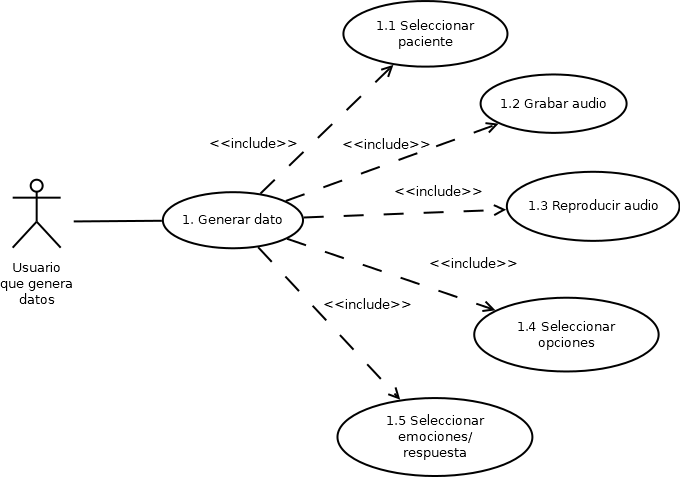
\includegraphics[width=\textwidth]{CU1}
	\caption{Caso de Uso 1.}
	\label{fig:cu1}
\end{figure}

\begin{figure}[H]
	\centering
	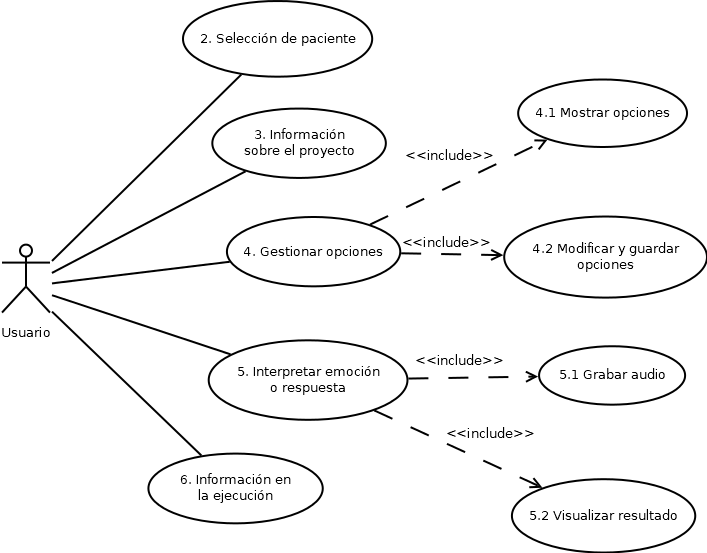
\includegraphics[width=\textwidth]{CU23456}
	\caption{Casos de Uso 2, 3, 4, 5 y 6.}
	\label{fig:cu}
\end{figure}

\subsection{Actores}
Los actores son las personas que interactuan con los elementos desarrollados y son los que definen los casos de uso de un proyecto. En este desarrollo podemos diferenciar los siguiente actores:
\begin{itemize}
	\item \textbf{Usuario que genera datos:} este usuario es el que interacciona con la aplicación para generar datos. Este usuario será los familiares, amigos y cuidadores más cercanos al paciente, que saben interpretar los sonidos que emite.
	\item \textbf{Usuario:} este usuario es el que interacciona con la aplicación de interpretación, y puede ser cualquier tipo de persona que quiera interpretar a una persona con parálisis cerebral gravemente afectada.
\end{itemize}
\subsection{Casos de uso}
\tablaSmallSinColores{Caso de uso 1:	Generar un dato.}{p{3cm} p{.75cm} p{9.5cm}}{tablaCU1}{
	\multicolumn{3}{p{10.25cm}}{\textbf{CU-1: Generar un dato.}} \\
}
{
	\textbf{Descripción}                            & \multicolumn{2}{p{10.25cm}}{El usuario sube un dato generado.} \\\hubu
	\textbf{Requisitos}                         	   & \multicolumn{2}{p{10.25cm}}{RF-5} \\\hubu
	\textbf{Actor}                         	   & \multicolumn{2}{p{10.25cm}}{Usuario que genera un dato.} \\\hubu
	\multirow{3}{3.5cm}{\textbf{Secuencia normal}}  & \textbf{Paso} & \textbf{Acción} \\\cline{2-3}
	& 1    & El usuario accede a la aplicación de generación de datos.\\\cline{2-3}
	& 2	   & El usuario selecciona al paciente. \\\cline{2-3}
	& 3    & El usuario rellena el audio, las opciones y las emociones o respuesta. \\\cline{2-3}
	& 4    & El usuario sube el dato generado. \\\hubu
	\textbf{Postcondiciones}                        & \multicolumn{2}{p{10.25cm}}{El correo con el dato se ha enviado correctamente.} \\\hubu
	\multirow{2}{3.5cm}{\textbf{Excepciones}}       & Paso & Acción \\\cline{2-3}
	& 4    & Si no se tiene conexión a Internet no se envía el dato, pero tampoco se elimina \\\hubu
	\textbf{Frecuencia}                             & Media \\\hubu
	\textbf{Importancia}                            & Crítico \\
}

\tablaSmallSinColores{Caso de uso 1.1:	Seleccionar un paciente.}{p{3cm} p{.75cm} p{9.5cm}}{tablaCU1.1}{
	\multicolumn{3}{p{10.25cm}}{\textbf{CU-1.1: Seleccionar un paciente.}} \\
}
{
	\textbf{Descripción}                            & \multicolumn{2}{p{10.25cm}}{El usuario selecciona y confirma un paciente.} \\\hubu
	\textbf{Precondiciones}                         & \multicolumn{2}{p{10.25cm}}{El usuario se encuentra en el menú principal de la aplicación de recogida de datos} \\\hubu
	\textbf{Requisitos}                         	   & \multicolumn{2}{p{10.25cm}}{RF-1, RF-1.1, RF1.2, RF-1.3.} \\\hubu
	\textbf{Actor}                         	   & \multicolumn{2}{p{10.25cm}}{Usuario que genera un dato.} \\\hubu
	\multirow{3}{3.5cm}{\textbf{Secuencia normal}}  & \textbf{Paso} & \textbf{Acción} \\\cline{2-3}
	& 1    & El usuario accede a la aplicación de generación de datos.\\\cline{2-3}
	& 2	   & El usuario despliega el \textit{spinner} para ver los posibles pacientes. \\\cline{2-3}
	& 3    & El usuario selecciona un paciente de entre los posibles. \\\cline{2-3}
	& 4    & El usuario confirma el paciente pulsando en el botón \textit{SEL.}. \\\hubu
	\textbf{Postcondiciones}                        & \multicolumn{2}{p{10.25cm}}{El usuario ha sido seleccionado y confirmado.} \\\hubu
	\textbf{Frecuencia}                             & Alta \\\hubu
	\textbf{Importancia}                            & Alta \\
}

\tablaSmallSinColores{Caso de uso 1.2:	Grabar audio.}{p{3cm} p{.75cm} p{9.5cm}}{tablaCU1.2}{
	\multicolumn{3}{p{10.25cm}}{\textbf{CU-1.2: Grabar audio.}} \\
}
{
	\textbf{Descripción}                            & \multicolumn{2}{p{10.25cm}}{El usuario graba el sonido emitido por un paciente.} \\\hubu
	\textbf{Precondiciones}                         & \multicolumn{2}{p{10.25cm}}{Hay un paciente seleccionado.} \\\hubu
	\textbf{Requisitos}                         	   & \multicolumn{2}{p{10.25cm}}{RF-4, RF-4.1, RF-4.3} \\\hubu
	\textbf{Actor}                         	   & \multicolumn{2}{p{10.25cm}}{Usuario que genera un dato.} \\\hubu
	\multirow{3}{3.5cm}{\textbf{Secuencia normal}}  & \textbf{Paso} & \textbf{Acción} \\\cline{2-3}
	& 1    & El usuario accede a la aplicación de generación de datos.\\\cline{2-3}
	& 2	   & El usuario selecciona al paciente. \\\cline{2-3}
	& 3    & El usuario pulsa el botón \textit{GRABAR AUDIO}. \\\cline{2-3}
	& 4    & El usuario pulsa el botón \textit{GRABAR} para comenzar a grabar. \\\cline{2-3}
	& 5    & El usuario pulsa el botón \textit{PARAR} para para la grabación.\\\hubu
	\textbf{Postcondiciones}                        & \multicolumn{2}{p{10.25cm}}{El audio está grabado y puede volver a grabarse pulsando el botón "GRABAR".} \\\hubu
	\textbf{Frecuencia}                             & Alta \\\hubu
	\textbf{Importancia}                            & Alta \\
}

\tablaSmallSinColores{Caso de uso 1.3:	Reproducir el audio.}{p{3cm} p{.75cm} p{9.5cm}}{tablaCU1.3}{
	\multicolumn{3}{p{10.25cm}}{\textbf{CU-1.3: Reproducir el audio.}} \\
}
{
	\textbf{Descripción}                            & \multicolumn{2}{p{10.25cm}}{El último audio grabado es reproducido.} \\\hubu
	\textbf{Precondiciones}                         & \multicolumn{2}{p{10.25cm}}{Existe un audio grabado, y el usuario se encuentra en la pantalla de grabación de audio.} \\\hubu
	\textbf{Requisitos}                         	   & \multicolumn{2}{p{10.25cm}}{RF-4.2} \\\hubu
	\textbf{Actor}                         	   & \multicolumn{2}{p{10.25cm}}{Usuario que genera un dato.} \\\hubu
	\multirow{3}{3.5cm}{\textbf{Secuencia normal}}  & \textbf{Paso} & \textbf{Acción} \\\cline{2-3}
	& 1    & El usuario pulsa el botón \textit{REPRODUCIR} y se comienza a reproducir el audio.\\\hubu
	\textbf{Postcondiciones}                        & \multicolumn{2}{p{10.25cm}}{El audio se reproduce, y si se vuelve a pulsar el botón vuelve a comenzar la reproducción.} \\\hubu
	\textbf{Frecuencia}                             & Baja \\\hubu
	\textbf{Importancia}                            & Media \\
}

\tablaSmallSinColores{Caso de uso 1.4:	Seleccionar las opciones adicionales.}{p{3cm} p{.75cm} p{9.5cm}}{tablaCU1.4}{
	\multicolumn{3}{p{10.25cm}}{\textbf{CU-1.4: Seleccionar las opciones adicionales.}} \\
}
{
	\textbf{Descripción}                            & \multicolumn{2}{p{10.25cm}}{El usuario quiere seleccionar las opciones relacionadas con el audio grabado.} \\\hubu
	\textbf{Precondiciones}                         & \multicolumn{2}{p{10.25cm}}{Estamos en la pantalla de selección de opciones y existe un audio grabado.} \\\hubu
	\textbf{Requisitos}                         	   & \multicolumn{2}{p{10.25cm}}{RF-3, RF-3.1} \\\hubu
	\textbf{Actor}                         	   & \multicolumn{2}{p{10.25cm}}{Usuario que genera un dato.} \\\hubu
	\multirow{3}{3.5cm}{\textbf{Secuencia normal}}  & \textbf{Paso} & \textbf{Acción} \\\cline{2-3}
	& 1    & El usuario selecciona las opciones apropiadas en ese momento.\\\hubu
	\textbf{Postcondiciones}                        & \multicolumn{2}{p{10.25cm}}{Las opciones se guardan, y si se vuelve acceder a la pantalla se cargan.} \\\hubu
	\textbf{Frecuencia}                             & Alta \\\hubu
	\textbf{Importancia}                            & Alta \\
}

\tablaSmallSinColores{Caso de uso 1.5:	Seleccionar las emociones o respuestas.}{p{3cm} p{.75cm} p{9.5cm}}{tablaCU1.5}{
	\multicolumn{3}{p{10.25cm}}{\textbf{CU-1: Seleccionar las emociones o respuestas.}} \\
}
{
	\textbf{Descripción}                            & \multicolumn{2}{p{10.25cm}}{El usuario quiere seleccionar las emociones o respuesta relacionadas con el audio.} \\\hubu
	\textbf{Precondiciones}                         & \multicolumn{2}{p{10.25cm}}{Estamos en la pantalla de selección de emociones o respuesta, con un audio grabado y unas opciones seleccionadas.} \\\hubu
	\textbf{Requisitos}                         	   & \multicolumn{2}{p{10.25cm}}{RF-2, RF-2.1, RF-2.2, RF-2.3 y RF-2.4.} \\\hubu
	\textbf{Actor}                         	   & \multicolumn{2}{p{10.25cm}}{Usuario que genera un dato.} \\\hubu
	\multirow{3}{3.5cm}{\textbf{Secuencia normal}}  & \textbf{Paso} & \textbf{Acción} \\\cline{2-3}
	& 1    & El usuario selecciona las emociones o respuesta relacionada.\\\hubu
	\textbf{Postcondiciones}                        & \multicolumn{2}{p{10.25cm}}{Lo seleccionado se guarda, y si se vuelve a entrar en la pantalla se cargarán estos datos.} \\\hubu
	\multirow{2}{3.5cm}{\textbf{Excepciones}}       & Paso & Acción \\\cline{2-3}
	& 1    & Si se selecciona emociones y respuestas no se puede aceptar. \\\cline{2-3} 
	& 1	   & Si se seleccionan las respuestas \textit{sí} y \textit{no}, no se permite aceptar. \\\cline{2-3}
	& 1    & Si no se selecciona nada no deja aceptar y salir de la pantalla.\\\hubu
	\textbf{Frecuencia}                             & Alta \\\hubu
	\textbf{Importancia}                            & Alta \\
}

\tablaSmallSinColores{Caso de uso 2:	Seleccionar paciente.}{p{3cm} p{.75cm} p{9.5cm}}{tablaCU2}{
	\multicolumn{3}{p{10.25cm}}{\textbf{CU-2: Seleccionar paciente.}} \\
}
{
	\textbf{Descripción}                            & \multicolumn{2}{p{10.25cm}}{El usuario selecciona el paciente con el cual quiere trabajar.} \\\hubu
	\textbf{Precondiciones}                         & \multicolumn{2}{p{10.25cm}}{Estar en la aplicación de interpretación, con conexión directa al servidor.} \\\hubu
	\textbf{Requisitos}                         	   & \multicolumn{2}{p{10.25cm}}{RF-1, RF-1.1, RF-1.2, RF-1.3 y RF-1.4} \\\hubu
	\textbf{Actor}                         	   & \multicolumn{2}{p{10.25cm}}{Usuario.} \\\hubu
	\multirow{3}{3.5cm}{\textbf{Secuencia normal}}  & \textbf{Paso} & \textbf{Acción} \\\cline{2-3}
	& 1    & El usuario despliega el \textit{spinner} para ver los posibles pacientes.\\\cline{2-3}
	& 2	   & El usuario selecciona al paciente con el que quiere trabajar.\\\hubu
	\multirow{2}{3.5cm}{\textbf{Excepciones}}       & Paso & Acción \\\cline{2-3}
	& 1	   & Si no se puede conectar con el servidor, saldrá un error 1. \\\hubu
	\textbf{Frecuencia}                             & Alta \\\hubu
	\textbf{Importancia}                            & Alta \\
}

\tablaSmallSinColores{Caso de uso 3:	Obtener información sobre el proyecto.}{p{3cm} p{.75cm} p{9.5cm}}{tablaCU3}{
	\multicolumn{3}{p{10.25cm}}{\textbf{CU-3: Obtener información sobre el proyecto.}} \\
}
{
	\textbf{Descripción}                            & \multicolumn{2}{p{10.25cm}}{El usuario tiene que poder ver información acerca del equipo de desarrollo.} \\\hubu
	\textbf{Precondiciones}                         & \multicolumn{2}{p{10.25cm}}{Estar en la aplicación de interpretación, con conexión directa al servidor.} \\\hubu
	\textbf{Requisitos}                         	   & \multicolumn{2}{p{10.25cm}}{RF-8} \\\hubu
	\textbf{Actor}                         	   & \multicolumn{2}{p{10.25cm}}{Usuario.} \\\hubu
	\multirow{3}{3.5cm}{\textbf{Secuencia normal}}  & \textbf{Paso} & \textbf{Acción} \\\cline{2-3}
	& 1    & El usuario, en el menú principal, pulsa el botón de información al lado del logo de la aplicación.\\\hubu
	\textbf{Postcondiciones}                        & \multicolumn{2}{p{10.25cm}}{El usuario se encuentra en la pantalla de información, puede salir pulsando el botón \textit{Aceptar}.} \\\hubu
	\textbf{Frecuencia}                             & Baja \\\hubu
	\textbf{Importancia}                            & Baja \\
}

\tablaSmallSinColores{Caso de uso 4:	Gestionar las opciones adicionales.}{p{3cm} p{.75cm} p{9.5cm}}{tablaCU4}{
	\multicolumn{3}{p{10.25cm}}{\textbf{CU-4: Gestionar las opciones adicionales.}} \\
}
{
	\textbf{Descripción}                            & \multicolumn{2}{p{10.25cm}}{El usuario quiere gestionar las opciones del paciente seleccionado.} \\\hubu
	\textbf{Precondiciones}                         & \multicolumn{2}{p{10.25cm}}{Estar en la aplicación de interpretación y haber seleccionado al paciente, con conexión directa al servidor.} \\\hubu
	\textbf{Requisitos}                         	   & \multicolumn{2}{p{10.25cm}}{RF-3 y RF-3.2} \\\hubu
	\textbf{Actor}                         	   & \multicolumn{2}{p{10.25cm}}{Usuario.} \\\hubu
	\multirow{3}{3.5cm}{\textbf{Secuencia normal}}  & \textbf{Paso} & \textbf{Acción} \\\cline{2-3}
	& 1    & El usuario, en el menú principal, pulsa el botón de \textit{Registro de Información}.\\\cline{2-3}
	& 2	   & El usuario visualiza las opciones guardadas para el paciente seleccionado. \\\cline{2-3}
	& 3    & El usuario puede modificar y guardar las opciones. \\\hubu
	\multirow{2}{3.5cm}{\textbf{Excepciones}}       & Paso & Acción \\\cline{2-3}
	& 2    &  Si no existe el fichero de opciones en el servidor, este devuelve un error 5.\\\hubu
	\textbf{Frecuencia}                             & Alta \\\hubu
	\textbf{Importancia}                            & Alta \\
}

\tablaSmallSinColores{Caso de uso 4.1:	Mostrar las opciones.}{p{3cm} p{.75cm} p{9.5cm}}{tablaCU4.1}{
	\multicolumn{3}{p{10.25cm}}{\textbf{CU-4.1: Mostrar las opciones.}} \\
}
{
	\textbf{Descripción}                            & \multicolumn{2}{p{10.25cm}}{El usuario al entrar en la pantalla visualizará las opciones guardadas para el paciente seleccionado.} \\\hubu
	\textbf{Precondiciones}                         & \multicolumn{2}{p{10.25cm}}{Estar en la pantalla de opciones.} \\\hubu
	\textbf{Requisitos}                         	   & \multicolumn{2}{p{10.25cm}}{RF-3 y RF-3.2} \\\hubu
	\textbf{Actor}                         	   & \multicolumn{2}{p{10.25cm}}{Usuario.} \\\hubu
	\multirow{3}{3.5cm}{\textbf{Secuencia normal}}  & \textbf{Paso} & \textbf{Acción} \\\cline{2-3}
	& 1    & El usuario visualiza las opciones guardas para el paciente seleccionado.\\\hubu
	\multirow{2}{3.5cm}{\textbf{Excepciones}}       & Paso & Acción \\\cline{2-3}
	& 1    &  Si no existe el fichero de opciones en el servidor, este devuelve un error 5.\\\hubu
	\textbf{Frecuencia}                             & Alta \\\hubu
	\textbf{Importancia}                            & Alta \\
}

\tablaSmallSinColores{Caso de uso 4.2:	Modificar y guardar las opciones.}{p{3cm} p{.75cm} p{9.5cm}}{tablaCU4.2}{
	\multicolumn{3}{p{10.25cm}}{\textbf{CU-4.2: Modificar y guardar las opciones.}} \\
}
{
	\textbf{Descripción}                            & \multicolumn{2}{p{10.25cm}}{El usuario modifica, y guarda o cancela los cambios.} \\\hubu
	\textbf{Precondiciones}                         & \multicolumn{2}{p{10.25cm}}{Estar en la pantalla de opciones.} \\\hubu
	\textbf{Requisitos}                         	   & \multicolumn{2}{p{10.25cm}}{RF-5} \\\hubu
	\textbf{Actor}                         	   & \multicolumn{2}{p{10.25cm}}{Usuario.} \\\hubu
	\multirow{3}{3.5cm}{\textbf{Secuencia normal}}  & \textbf{Paso} & \textbf{Acción} \\\cline{2-3}
	& 1    & El usuario visualiza las opciones para el paciente seleccionado.\\\cline{2-3}
	& 2	   & El usuario modifica alguna de las opciones, habilitando así el botón \textit{Guardar}. \\\cline{2-3}
	& 3    & El usuario guarda o cancela los cambios. \\\hubu
	\textbf{Postcondiciones}                        & \multicolumn{2}{p{10.25cm}}{Si el usuario ha decidido guardar, los cambios se realizan en el servidor.} \\\hubu
	\multirow{2}{3.5cm}{\textbf{Excepciones}}       & Paso & Acción \\\cline{2-3}
	& 1    &  Si no existe el fichero de opciones en el servidor, este devuelve un error 5.\\\cline{2-3}
	& 3    & Si no hay conexión con el servidor, se muestra un error 1. \\\hubu
	\textbf{Frecuencia}                             & Media \\\hubu
	\textbf{Importancia}                            & Alta \\
}

\tablaSmallSinColores{Caso de uso 5:	Interpretar emoción o respuesta.}{p{3cm} p{.75cm} p{9.5cm}}{tablaCU5}{
	\multicolumn{3}{p{10.25cm}}{\textbf{CU-5: Interpretar emoción o respuesta.}} \\
}
{
	\textbf{Descripción}                            & \multicolumn{2}{p{10.25cm}}{El usuario quiere interpretar las emociones y las respuestas de los pacientes.} \\\hubu
	\textbf{Precondiciones}                         & \multicolumn{2}{p{10.25cm}}{Estar en la aplicación de interpretación con un paciente seleccionado, y con conexión directa al servidor.} \\\hubu
	\textbf{Requisitos}                         	   & \multicolumn{2}{p{10.25cm}}{RF-6, RF-6.1 y RF-6.2.} \\\hubu
	\textbf{Actor}                         	   & \multicolumn{2}{p{10.25cm}}{Usuario.} \\\hubu
	\multirow{3}{3.5cm}{\textbf{Secuencia normal}}  & \textbf{Paso} & \textbf{Acción} \\\cline{2-3}
	& 1    & El usuario, en el menú principal, pulsa el botón \textit{Qué quiero decir}.\\\cline{2-3}
	& 2	   & El usuario selecciona el tipo de interpretación que quiere hacer. \\\cline{2-3}
	& 3    & El usuario graba el audio que quiere interpretar. \\\cline{2-3}
	& 4    & El usuario visualiza y escucha el resultado. \\\hubu
	\multirow{2}{3.5cm}{\textbf{Excepciones}}       & Paso & Acción \\\cline{2-3}
	& 1    & Si no se puede conectar con el servidor, saldrá un error 1. \\\cline{2-3}
	& 4	   & Si no se puede conectar con el servidor, saldrá un error 1.\\\cline{2-3}
	& 4    & Si no existe un modelo válido para el paciente error 8. \\\hubu
	\textbf{Frecuencia}                             & Alta \\\hubu
	\textbf{Importancia}                            & Crítica \\
}

\tablaSmallSinColores{Caso de uso 5.1:	Grabar audio.}{p{3cm} p{.75cm} p{9.5cm}}{tablaCU5.1}{
	\multicolumn{3}{p{10.25cm}}{\textbf{CU-5.1: Grabar audio.}} \\
}
{
	\textbf{Descripción}                            & \multicolumn{2}{p{10.25cm}}{El usuario tiene que poder grabar el audio que quiere interpretar.} \\\hubu
	\textbf{Precondiciones}                         & \multicolumn{2}{p{10.25cm}}{Haber seleccionado un paciente, y estar en la pantalla de selección de interpretación con conexión directa al servidor.} \\\hubu
	\textbf{Requisitos}                         	   & \multicolumn{2}{p{10.25cm}}{RF-5} \\\hubu
	\textbf{Actor}                         	   & \multicolumn{2}{p{10.25cm}}{Usuario.} \\\hubu
	\multirow{3}{3.5cm}{\textbf{Secuencia normal}}  & \textbf{Paso} & \textbf{Acción} \\\cline{2-3}
	& 1    & El usuario selecciona el tipo de interpretación.\\\cline{2-3}
	& 2	   & El usuario graba el audio que quiere interpretar.\\\hubu
	\textbf{Postcondiciones}                        & \multicolumn{2}{p{10.25cm}}{El audio que ha grabado se puede reproducir, pulsando el botón \textit{Escuchar}, o se puede volver a grabar pulsando \textit{Grabar}.} \\\hubu
	\textbf{Frecuencia}                             & Alta \\\hubu
	\textbf{Importancia}                            & Crítica \\
}

\tablaSmallSinColores{Caso de uso 5.2:	Visualizar y escuchar el resultado.}{p{3cm} p{.75cm} p{9.5cm}}{tablaCU5.2}{
	\multicolumn{3}{p{10.25cm}}{\textbf{CU-5.2: Visualizar y escuchar el resultado.}} \\
}
{
	\textbf{Descripción}                            & \multicolumn{2}{p{10.25cm}}{El usuario quiere visualizar el resultado y poder volver a escuchar el audio relacionado con este resultado.} \\\hubu
	\textbf{Precondiciones}                         & \multicolumn{2}{p{10.25cm}}{Estar en la pantalla de grabación del audio, con un audio ya grabado y con conexión directa al servidor.} \\\hubu
	\textbf{Requisitos}                         	   & \multicolumn{2}{p{10.25cm}}{RF-6, RF-6.1, RF-6.2 y RF-4.4.} \\\hubu
	\textbf{Actor}                         	   & \multicolumn{2}{p{10.25cm}}{Usuario.} \\\hubu
	\multirow{3}{3.5cm}{\textbf{Secuencia normal}}  & \textbf{Paso} & \textbf{Acción} \\\cline{2-3}
	& 1    & El usuario pulsa el botón \textit{Entender} para ver el resultado.\\\cline{2-3}
	& 2	   & El usuario visualiza y escucha el resultado. \\\cline{2-3}
	& 3    & El usuario puede volver a escuchar el audio relacionado con ese resultado pulsando el botón \textit{Escuchar}. \\\hubu
	\textbf{Postcondiciones}                        & \multicolumn{2}{p{10.25cm}}{El correo con el dato se ha enviado correctamente.} \\\hubu
	\multirow{2}{3.5cm}{\textbf{Excepciones}}       & Paso & Acción \\\cline{2-3}
	& 2    & Si no se tiene conexión con el servidor, error 1. \\\cline{2-3}
	& 2    & Si no existe el modelo entrenado o está dentro del grupo de resultado aleatorios, error 8. \\\hubu
	\textbf{Frecuencia}                             & Alta \\\hubu
	\textbf{Importancia}                            & Crítica \\
}

\tablaSmallSinColores{Caso de uso 6:	Información en la ejecución.}{p{3cm} p{.75cm} p{9.5cm}}{tablaCU6}{
	\multicolumn{3}{p{10.25cm}}{\textbf{CU-6: Información en la ejecución.}} \\
}
{
	\textbf{Descripción}                            & \multicolumn{2}{p{10.25cm}}{El usuario quiere tener información sobre las acciones que hacen los botones de la aplicación.} \\\hubu
	\textbf{Precondiciones}                         & \multicolumn{2}{p{10.25cm}}{-} \\\hubu
	\textbf{Requisitos}                         	   & \multicolumn{2}{p{10.25cm}}{RF-5} \\\hubu
	\textbf{Actor}                         	   & \multicolumn{2}{p{10.25cm}}{Usuario.} \\\hubu
	\multirow{3}{3.5cm}{\textbf{Secuencia normal}}  & \textbf{Paso} & \textbf{Acción} \\\cline{2-3}
	& 1    & Si el usuario pulsa algún botón de información se abrirá un diálogo explicativo en lectura fácil, además se reproducirá por audio. \\\hubu
	\textbf{Frecuencia}                             & Baja \\\hubu
	\textbf{Importancia}                            & Baja \\
}